\scanpage{41}
\noindent\hfill atkin \mspage{1}\margin{\handwritten{\figure{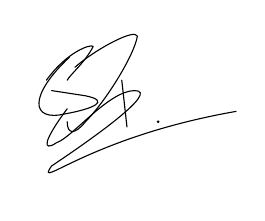
\begin{tikzpicture}[x=.33mm,y=-.33mm,line cap=round,line join=round]
\draw (4,18) .. controls (12,7) and (21,4) .. (22,5) .. controls (19,11) and (13,16) .. (12,18);
\draw (15,13) .. controls (23,6) and (38,-2) .. (39,1) .. controls (38,8) and (27,26) .. (19,34) .. controls (15,39) and (12,39) .. (12,34);
\draw (13,9) .. controls (-3,24) and (-2,34) .. (11,31) .. controls (22,29) and (29,26) .. (19,24) -- (6,22);
\draw (12,29) .. controls (3,41) and (2,46) .. (8,42) .. controls (14,40) and (28,22) .. (38,22) .. controls (48,22) and (21,41) .. (6,51) .. controls (-1,61) and (20,40) .. (77,30);
\draw (33,18) -- (35,36);
\fill (47,34) circle (.55);
\end{tikzpicture}}}}

\begin{center}
CONGRUENCES FOR MODULAR FORMS\quad \handwritten{(1968)}

by

A.O.L.ATKIN*
\end{center}

\handwritten{\figure{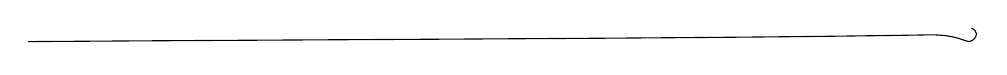
\begin{tikzpicture}[x=\linewidth,y=1mm,line cap=round]
\draw (0,0) .. controls (.35,.3) and (.72,.4) .. (.94,.85) .. controls (.98,1) and (.982,-.55) .. (.99,.25) .. controls (.994,.65) and (.995,1.35) .. (.988,1.7);
\end{tikzpicture}}}

\noindent * Research Fellow of the Atlas Computer Laboratory

\handwritten{\figure{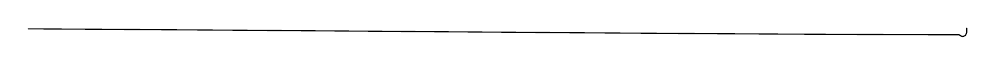
\begin{tikzpicture}[x=\linewidth,y=1mm,line cap=round]
\draw (0,.3) .. controls (.32,.08) and (.72,-.4) .. (.975,-.45) .. controls (.981,-1.05) and (.984,-.36) .. (.983,.38);
\end{tikzpicture}}}

\noindent 1. Introduction. This paper describes in general terms my attempts to extend and generalise congruence properties of modular forms with the aid of a computer(the ICT Atlas 1 computer of the Science Reserach Council at Chilton). The main practical conclusion can be stated simply: working in continuous direct contact with a large and powerful computer establishment has led to results far beyond my original expectations. Accordingly it seems worth while to try and give here some account of the actual process of discovery as it appeared to me at the time,which involves in effect a description of the work in reverse logical order; and to publish elsewhere the full mathematical details and a ``logical'' exposition based on the work in reverse order of time.

I have used Atlas to obtain a number of results,some of which are more interesting computationally than the present work. But in so far as the computer's function is to assist research,what matters is the final mathematical result rather than(to be fanciful) the machine's personal enjoyment of the tasks it has been ordered to perform. I am perfectly clear that the work described in this paper represents the most significant use I have made of Atlas. It might in theory have been possible to arrive at some of these results by \uline{a priori} reasoning; certainly the \unsure{.}cases where the proofs are complete require in the event no more computation than a few hours' hand work. But I would not myself have been able to conjecture the possibility of such results without the evidence provided by the computer.

I should like to thank the Director,Dr. J.Howlett,and my other colleagues at the Atlas Computer Laboratory for the frequent help they have given me. In particular I have had many valuable discussions

% archive sheet number: 40
